\chapter{Methods}
\label{ch:methods}
We've decided on the following approach for the assisted navigation. We use four different ToF ranging sensors each mounted on one side and pointing in either negative or positive x-direction, or in either negative or positive y-direction (\cref{fig:sketch}). These sensors send the ranging data to the \textit{pixhawk} autopilot, in which, w.t.h. of a potential field, the repulsive force is computed. The force is converted into corrective attitude angles and send to the attitude controller (\cref{fig:approach}). Eventually, the drone should push itself away from the obstacle.\\\\

The overall methodology of the thesis can be split into the following steps:
\begin{enumerate}
	\item Evaluation of the \textit{VL53L0X} ToF Ranging Sensor with a \textit{mbed LPC1768} microcontroller on its potential use for obstacle avoidance on a MAV (\cref{sec:ranging sensor})
	\item Integration of four \textit{VL53L0X} sensors on the pixhawk autopilot
	\item Implementation of a potential field on the \textit{pixhawk}.
\end{enumerate}

\begin{figure}
	\centering
	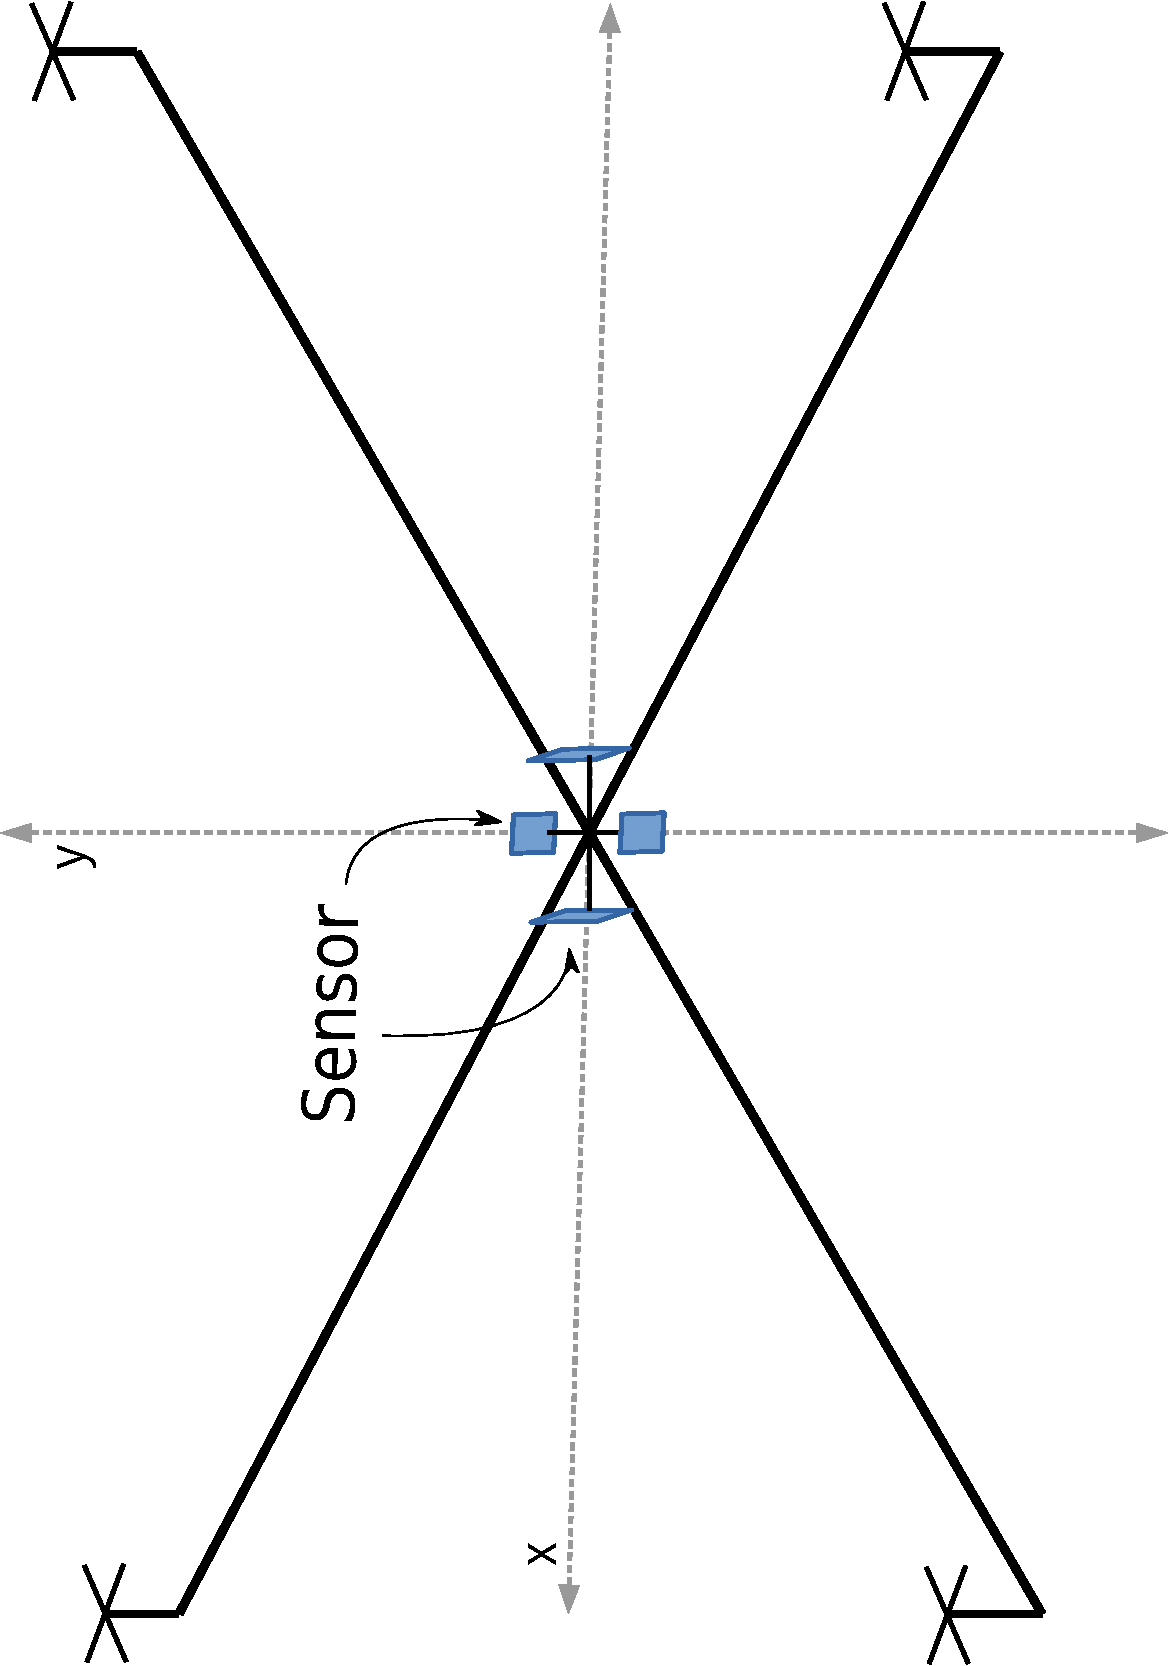
\includegraphics[width=0.4\linewidth, angle = 270]{pictures/mav_sketch.pdf}
	\caption{Sketch of the sensor's setup on the MAV.}
	\label{fig:sketch}
\end{figure}

\begin{figure}
	\centering
	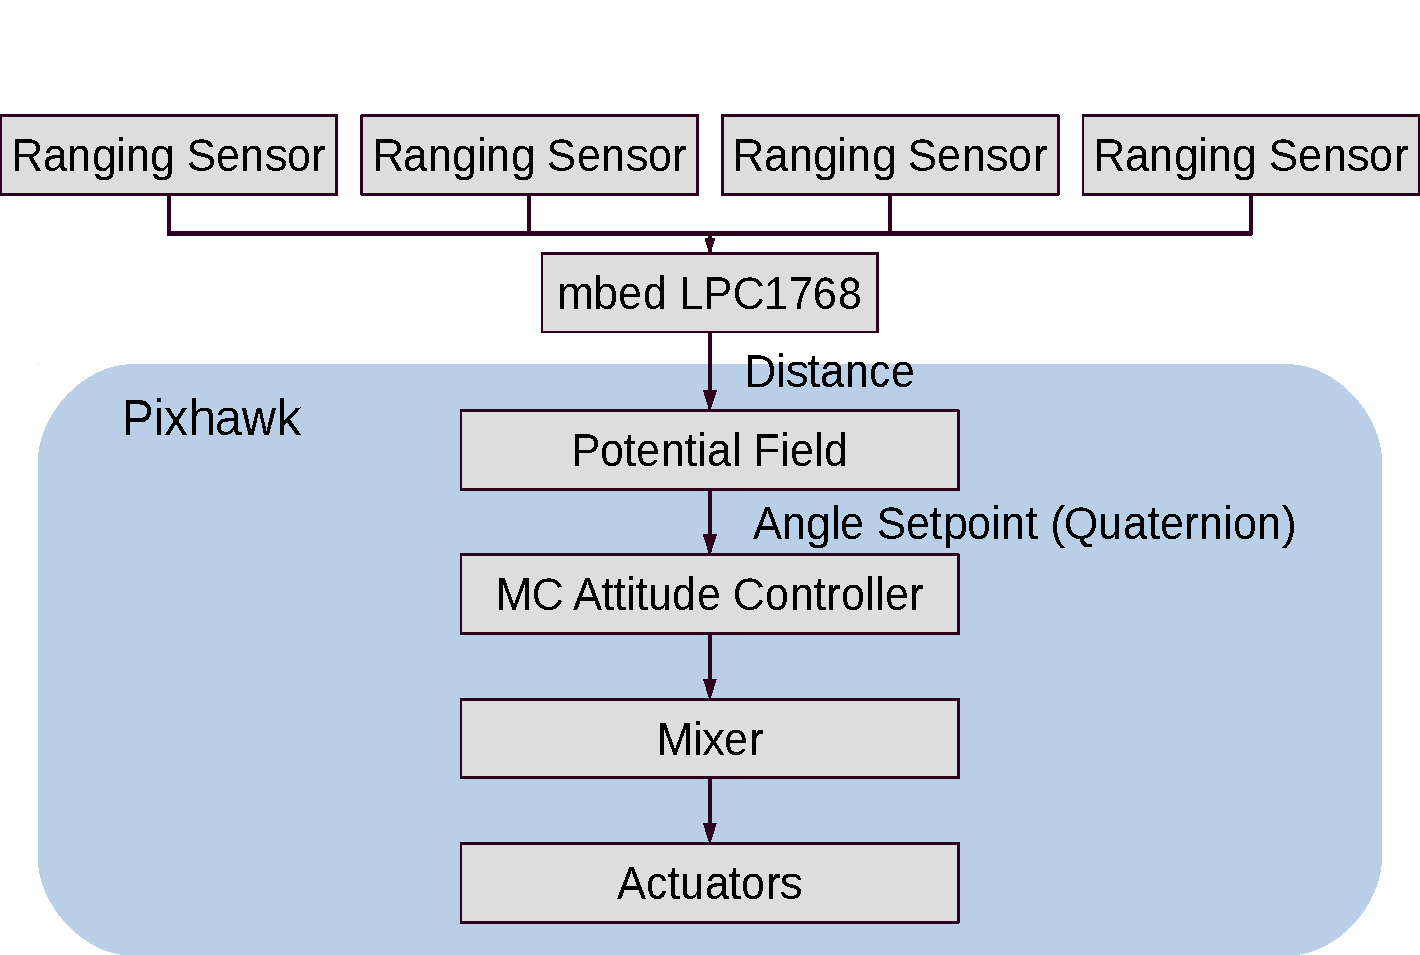
\includegraphics[width=0.8\linewidth]{pictures/approach.pdf}
	\caption{Approach we have chosen for the obstacle avoidance.}
	\label{fig:approach}
\end{figure}

\section{Ranging Sensor}
\label{sec:ranging sensor}
A major constraint for MAVs is the payload and the available power, thus, we needed a low power and on the same time lightweight ranging sensor. We've opted for the \textit{VL53L0X} ToF Ranging Sensor developed by \textit{STMicroelectronics} (\cref{fig:sensor}) for the distance measurements due to its low power consumption and its lightweight.   For the evaluation we connected the sensor via I2C to a \textit{mbed LPC1768} microcontroller. The sensor has a range of \unit[0]{mm} up to \unit[2]{m} under optimal conditions, i.e. no infrared radiation.  The sensor allows four different modes to be used (\cref{tab:profile}). To facilitate the integration we use the \textit{53L0-SATEL-I1} satellite board (\cref{(fig:satellite)}). The \textit{VL53L0X} sensor comes with a Application Programming Interface (API) which allows to control of the VL53L0X Firmware like initialisation/calibration, ranging Start/Stop, choice of accuracy and choice of ranging mode. If the sensor is not able to make a measurement or the target is outside of its range, the API return a value greater than 8000.\\
\begin{figure}
	\centering
	\begin{minipage}{0.4\textwidth}
		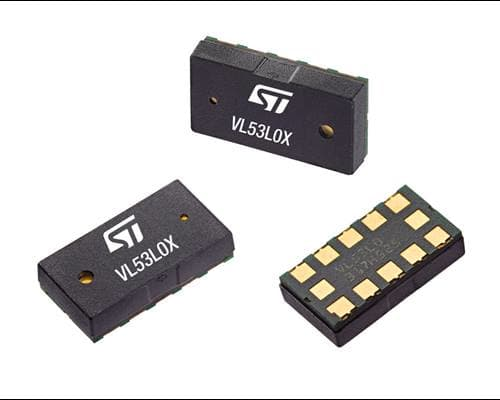
\includegraphics[width=0.9\linewidth]{pictures/vl53l0x_article2.jpg}
		\caption{\textit{VL53L0X} ranging and gesture detection sensor}
		\label{fig:sensor}
	\end{minipage}
	\quad
	\begin{minipage}{0.4\textwidth}
		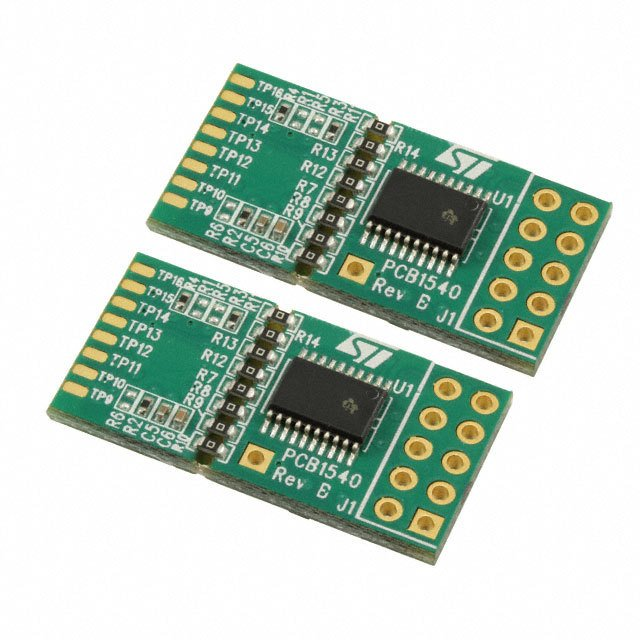
\includegraphics[width=0.9\linewidth]{pictures/53L0-SATEL-I1.jpg}
		\caption{\textit{53L0-SATEL-I1} Satellite boards based on \textit{VL53L0X} ranging and gesture detection sensor}
		\label{fig:satellite}
	\end{minipage}
\end{figure}
\begin{table}[]
	\centering
	\caption{Range profile}
	\label{tab:profile}
	\resizebox{\textwidth}{!}{%
		\begin{tabular}{|c|c|c|c|}
			\hline
			\textbf{Range Profile} & \textbf{Range Timing Budget} & \textbf{Typical Performance} & \textbf{Typical Application}                                                             \\ 
			\specialrule{.2em}{.1em}{.1em} 
			Default Mode           & 30 ms                        & 1.2 m                        & Standard                                                                                 \\ \hline
			High Accuracy          & 200 ms                       & 1.2 m                        & Precise Measurement                                                                      \\ \hline
			Long Range             & 33 ms                        & 2 m                          & \begin{tabular}[c]{@{}c@{}}Long Rangin,\\  only for dark conditions (no IR)\end{tabular} \\ \hline
			High Speed             & 20 ms                        & 1.2 m                        & \begin{tabular}[c]{@{}c@{}}High Speed, \\ where accuracy is not important\end{tabular}   \\ \hline
		\end{tabular}%
	}
\end{table}
We evaluated the sensor's performance using different target surfaces and under different lightning conditions. During the measurements we varied the angles and distance relative to the target. For the ground truth measurement we used a yardstick and a protractor. We conducted 100 measurements for every measurement setup. The surfaces used for the evaluation were a white plastered wall, a concrete wall and a wooden wall (\cref{fig:surfaces}).\\
The sensor uses IR for the measurement. Another strong IR source, e.g. the sun, reduces the accuracy and might even obstruct the sensor from making a measurement. To get reliable data, first, we filtered out the failed measurements, i.e. removing all data points with a value greater than 8000, and, second, rejected outliers w.t.h. of the Mahalonobis distance and filtered the remaining data points with a Kalman filter (\cref{alg:filter}). For the filter, we assumed constant distance in the process model:
\begin{equation}
\label{eq:filter}
\begin{split} 
x_k & = x_{k-1} \\
y_k & = x_k + v_k
\end{split}
\end{equation}
The noise process $v_k$ is white, zero-mean, uncorrelated, and has known covariance matrix  $R_k$.\\
The assumption of constant distance is only valid for the evaluation of the sensor. In case of a moving sensor or target a dynamic process model has to be developed. Further, a IMU should be used for the a priori state estimate. The VL53L0X sensor fused with a IMU has a faster update rate and performs more accurate. \\

\begin{algorithm}
	\caption{Filter}\label{alg:filter}
	\begin{algorithmic}[1]
		\Procedure{FILTER}{ }
		\State $y_{data}\gets \text{raw data points}$ 
		\State Filter out corrupted data points from $y_{data}$ \\
		\textit{Initzialization:}
		\State $\hat{x}^+_0\gets\text{initial measurement }y_{data}(0)$
		\State $R_k\gets\unit[27^2]{mm^2}$ \Comment{variance of the measurements}
		\State $P^+_0\gets \unit[30]{mm^2}$ \Comment{got this value from tuning}
		\For{ each $k = (0, \text{ number of data point]}$}	
		\State  $P^-_k \gets \text{Covariance of estimation error}$
		\State	$K_k \gets \text{Kalman gains}$
		\EndFor \\
		\textit{State Estimation:}	 
		\For{ each $k = (0, \text{ number of data point]}$}
		\State \Call{Mahal}{$y_{data,k}$} \Comment{Outliers rejection with mahalanobis distance}
		\State $\hat{x}^-_k \gets \text{a priori state estimate}$
		\State $\hat{x}^+_k \gets \text{a posteriori state estimate}$
		\EndFor
		\State \Return $\hat{x}^+_k$
		\EndProcedure
		
	\end{algorithmic}
\end{algorithm}





\section{Pixhawk}
\label{sec:pixhawk}
We use a \textit{pixhawk mRo} as a autopilot. The  \\
First, we tried to connect four different VL53L0X sensors to the pixhawk via I2C. Compiling the firmware on the pixhawk resulted in a flash overflow due to the large sensor API. The API is essential for the initialization and calibration of the VL53L0X sensors. To circumvent this problem, we connect the four sensors to the previously used mbed LPC1768 microcontroller and send the data from the mbed microcontroller to the pixhawk via I2C. Therewith, we can compile the API on the mbed microcontroller and on the pixhawk we just have to read the data. We read the data with the help of a self written driver. The only task of the driver is to continuously read the ranging data send by the mbed and publish the data to our self written topic. The topic is then subscribed by a self-written module in which attitude corrective angles $q_{pf}$ are calculated with the help of a potential field (\cref{subs:potential field}). These corrective angles are published to a new topic. This topic is subscribed by the multi-copter attitude controller on the pixhawk. In the attitude controller, the potential field attitude corrective angles $q_{sp}$ are added to the attitude set-points $q_{sp}$ (\cref{alg:px4}).

\begin{algorithm}
	\caption{Pixhawk}\label{alg:px4}
	\begin{algorithmic}[1]
		\Procedure{PIXHAWK}{ }
		\State Driver reads ranging data from I2C bus 
		\State Publish ranging data to topic \textit{VL53L0X}
		\State Module \textit{Potential Field} subscribes to topic \textit{VL53L0X}
		\State $y_{data}\gets \text{ranging data from topic \textit{VL53L0X}}$
		\State $q_{pf} \gets \text{corrective attitude angles calculated w.t.h of a potential field}$
		\State publish $q_{pf}$ to topic \textit{Potential Field}
		\State \textit{Multicopter Attitude Controller} subscribes to topic \textit{Potential Field}
		\State $q_{sp}\gets q_{sp}+q_{pf}$
		\EndProcedure
	\end{algorithmic}
\end{algorithm}


\subsection{Potential Field}
\label{subs:potential field}
The basic idea behind all potential field approaches is that the robot is attracted toward the goal, while being repulsed by the obstacles. For our system, we're only interested in the repulsive potential $U_{rep}$. This potential should be very strong when the system is close to a obstacle and on the same time should not be influenced by obstacle far away. One example of such a repulsive field is:
\begin{equation}
\label{eq:pot field}
\centering
U_{rep}(q)=\begin{cases}
\dfrac{1}{2}k_{rep}\left(\dfrac{1}{\rho (q)}-\dfrac{1}{\rho_0}\right)^2 & \text{if } \rho(q)\leq\rho_0 \\
0 & \text{if } \rho(q)\geq\rho_0 \text{ ,}
\end{cases}
\end{equation}
where $k_{rep}$ is a scaling factor, $\rho(q)$ is the minimal distance from to the object to the system position $q$ and $\rho_0$ is the distance of influence of the object. The repulsive potential function is positive or zero and tends to infinity as $q$ gets closer to the object.\\
If the object boundary is convex and piecewise differentiable, $\rho(q)$ is differentiable everywhere in the free configuration space. This leads to the repulsive force $F_{rep}$:
\begin{equation}
\begin{split}
F_{rep} &=-\Delta U_{rep}(q)\\
&=	\begin{cases}
k_{rep}\left(\dfrac{1}{\rho(q)}-\dfrac{1}{\rho_0}\right)\dfrac{1}{\rho^2(q)}\dfrac{q-q_{obstacle}}{\rho(q)} & \text{if }\rho(q)\leq\rho_0\\
0 & \text{if }\rho(q)\geq\rho_0
\end{cases}
\end{split}
\end{equation}

